\documentclass[../main.tex]{subfiles}
\graphicspath{{\subfix{../images/}}}
\begin{document}
	
\chapter{Determination of pointing requirements}

STEP is to do photometry of stars. Photometry is an astronomical method that is explained in detail in the following sections, is used to search for exoplanet transits. It requires time-series data of star fluxes, by the acquisition of images of stars. Starlight can be approximated as a point source of light, and illuminates a spot on the CCD chip face. This light has a so-called point spread function, which qualitatively describes the spreading of the light from the point source. This smearing phenomenon is usually due to the optics that image the light onto the chip, and depends on the focus of the image. For an image in perfect focus, the spot will be small, well defined (sharp), and show a diffraction pattern. In any case, the light will display some degree of spatial spread. This poses an issue for time-series data.

In general, a CCD detector does not have a uniform response to light across the chip. This can be due to non-flatness, and differences in pixel by pixel response to light, but can also be due to the way the chip is constructed. Consider for example figure \ref{fig:ccdreadreg}. The red area represents the pixel area. Between photosensitive channels are columns that separate the channels, such that we can distinguish pixels. Any photons incident on the part of the chip will not be included in the measured signal. Consider now light incident from a star, with a point spread function. The light is usually defocused and illuminates a subset of the pixels on the CCD chip. 

If the satellite moves during the acquisition of the time-series data, the light centroid (the center of the light spot) will move on the chip. This can result in more of the light being incident on non-sensitive parts of the chip, or on pixels of different sensitivity to incoming photons, and the result is a temporal flux that varies. If we are to study variations of the flux in a star system, such as an exoplanet transit, which is a dip in the flux levels as a function of time, we might mistake variations in the flux due to movements, as actual changes in the stellar system. These considerations, together with mission requirements, pose constraints on the pointing ability of the spacecraft.

In this chapter, we shall investigate the pointing requirements of the detector, posed when the detector is to be used in photometry. The relevant requirements have been defined above in table \ref{table:missionspecs}, and an experimental procedure to investigate the pointing requirements that arise from these scientific requirements will be outlined in the following. First photometric measurement methods are outlined, and then the experimental setup and procedure with results and conclusions will follow.

\section{Photometry}
In astronomy, \textbf{photometry} is the act of measuring the flux of an astronomical object, such as a star. For an astronomical mission such as STEP, photometric measurements are used in transit measurements, where the relative temporal flux of a star is studied. A specific kind of photometry, \textbf{differential photometry}, is used and will be explained in the following. 

\subsection{Differential photometry}\label{sec:diffphot}
\textbf{Differential photometry} is the estimation of the relative flux between a target star and a reference star, or field of stars. If an astronomical mission, such as STEP, is to search for exoplanets via the transit method, time series flux measurements of the light from the star are utilized. For this kind of data, we study the relative changes in the flux from the star. Hence, we do not need to know the absolute magnitude of the flux. Differential photometry fulfills this exact purpose, by estimating the flux of a target star relative to that of a reference star. This is useful since any experimental errors from the instruments used, common to the two sources of light, will be removed from the data. Differential photometry is usually done using aperture photometry which is outlined in the next section.

\subsection{Aperture photometry}\label{sect:apphotmeth}
To study the relative temporal flux of a single target star, \textbf{aperture photometry} is used. This technique utilizes a so-called \textbf{aperture} to single out the light from a star. The aperture is a circular selection of the sky that completely encompasses the light from the star. The light is assumed to be distributed around a \textbf{centroid}, denoting the \textit{'center of mass of the stars light'}. This centroid is estimated using the Python3 library Astropy PhotoUtils\cite{larry_bradley_2020_4044744} and represents the position of the spot on the CCD plane. We must also take into account the background light in the image, resulting from other stars, or for a telescope on earth, resulting from scattering in the sky. We may do this by drawing an \textbf{annulus} of inner radius greater than the aperture. This concept is illustrated in figure \ref{fig:aperture}.

\begin{figure}[h!]
	\centering
	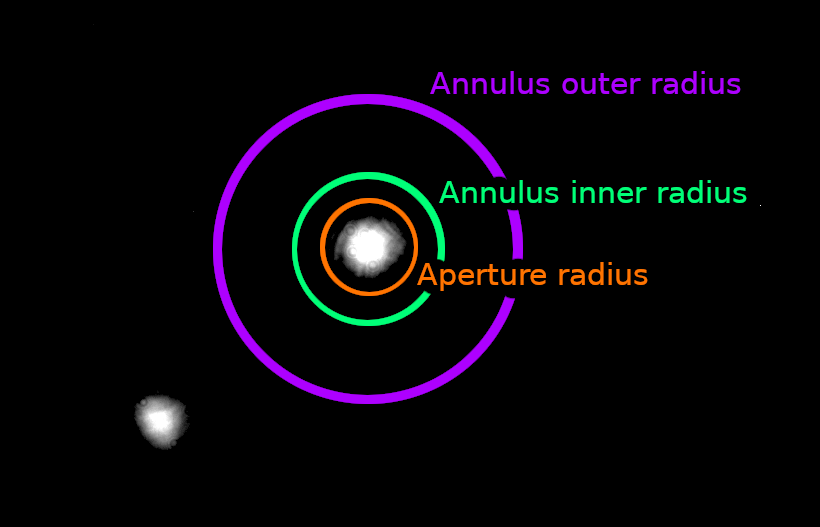
\includegraphics[width	=0.8\textwidth]{aperturespots.png}
	\caption{An outcrop of an image of two spots shined on a CCD, resulting from the experimental setup described in section \ref{sect:diffsetup}. An aperture is selected for the target star, as well as an appropriate annulus.}
	\label{fig:aperture}
\end{figure}

In order to determine the temporal flux of the target star, at first, the flux within the aperture is determined. This is done by adding, on a pixel-by-pixel basis, the ADU values. The same is then done for the annulus. The latter value is divided by the annulus area, yielding the value of the background per pixel. 
\begin{equation}
	\textbf{Background ADU/pixel} = \frac{\sum_\text{pixels inside annulus} \text{ADU in each pixel}}{\text{Area of annulus}}
\end{equation}
It is assumed that the background level in the annulus is the same as that within the aperture, such that after having found the mean pixel value of the background, we can multiply it with the area of the aperture and subtract this quantity from the counts inside the aperture, to estimate the true flux (in ADU). This is also sometimes called the \textbf{integral flux}.
\begin{equation}
	\textbf{Integral flux} = \sum_\text{pixels in aperture} \frac{\text{ADU}}{\text{pixel}} - \left(\frac{\text{Background ADU}}{\text{pixel}}\right) \cdot \text{(Area of aperture)}
\end{equation}
The method just outlined can be automated using the Python3 Library AStropy Photoutils \cite{larry_bradley_2020_4044744}, where library functions enable the construction of apertures and annuli from appropriately chosen (by the user), radii for the annuli, and coordinates for the aperture centers. These quantities are qualitatively estimated from the first image in the data series and held constant throughout the entire analysis, where the centroid only moves on a sub-pixel level.

\section{Attitude determination and control systems}
To motivate the discussions on pointing requirements, a brief explanation of the \textbf{attitude determination and control system} is in order. The stability requirement that is to be derived below in the proceeding analysis, is directly included in the attitude control system of the spacecraft. 
The \textbf{attitude} of a spacecraft is its orientation in space \cite{adcsbook}. 
\textbf{Attitude determination} is the act of determining this orientation. This is done by computing the orientation and position of the spacecraft, usually with respect to an inertial frame of reference, such as the earth or sun. This process typically involves the use of data from several different sensors on the spacecraft. These sensors are detectors such as sun sensors, earth horizon sensors, star trackers, and magnetorquers, among many others. Most sensors measure an angle with respect to the sensor. The principle behind this is illustrated in figure \ref{fig:sensorcones}. 

\begin{figure}[h!]
	\centering
	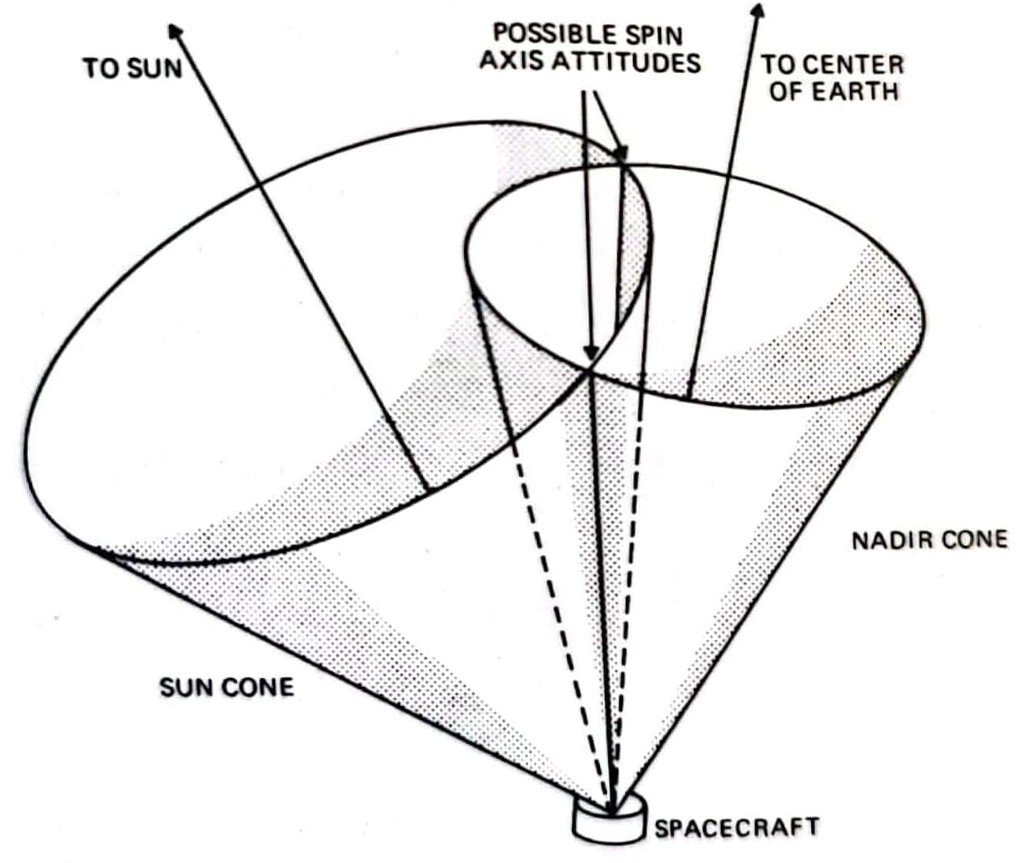
\includegraphics[width = 0.6\textwidth]{sensorcones.png}
	\caption{An example of attitude determination \cite{adcsbook}. Two sensors are used, a sun sensor, and an earth horizon sensor. The nadir cone is a cone around the nadir vector, which is an inertial vector pointing towards the earth at all times. Both of these sensors measure an angle with respect to the spacecraft and vectors of the sun and earth measured. The angles lie on a cone around the sensed direction. The intersections of these two cones are the possible attitudes, where usually one may be ruled out by using prior attitude history.}
	\label{fig:sensorcones}
\end{figure}

\textbf{Attitude control} is the act of controlling the attitude, usually by stabilizing it and predicting future attitudes, or by performing maneuvers to obtain a new desired attitude. This can be achieved using \textbf{torquers} such as external thrusters, magnetorquers, and reaction wheels among others. 

The process of attitude determination and control is crucial and very important to a space mission. Solar arrays must be pointed at the sun, antennas for data downlink to earth must be pointed toward the ground station, and payloads must be oriented such that measurements can be performed as desired. In the present case of STEP, the telescope must be pointed towards a field of stars. As is evident from the previous discussion, this is very important for photometry. Both the absolute and differential measurements are affected by drifts in the flux due to drifts in the attitude, and we should take great care in stabilizing the spacecraft during the acquisition of flux data from stars.

An overview of the ADCS implementation can be seen in figure \ref{fig:acsblockdiag}. This is a very basic example of an attitude determination \textbf{control flow}. The attitude is measured by sensors. This data is then fed into the \textbf{onboard computer} (OBC). The OBC must then determine if the attitude is to be controlled via the application of a torque. Here \textit{disturbances} refer to any external torques from the environment that may, or may not be, undesirable. Examples of these are torques induced by the solar radiation pressure or differences in the earth's gravitational field. The pointing requirements that will be derived in the following sections are input directly into this control flow. After attitude determination, the OBC must determine if we have drifted too far from the initial attitude. The OBC must then correct the attitude following this measurement. 

\begin{figure}[h!]
	\centering
	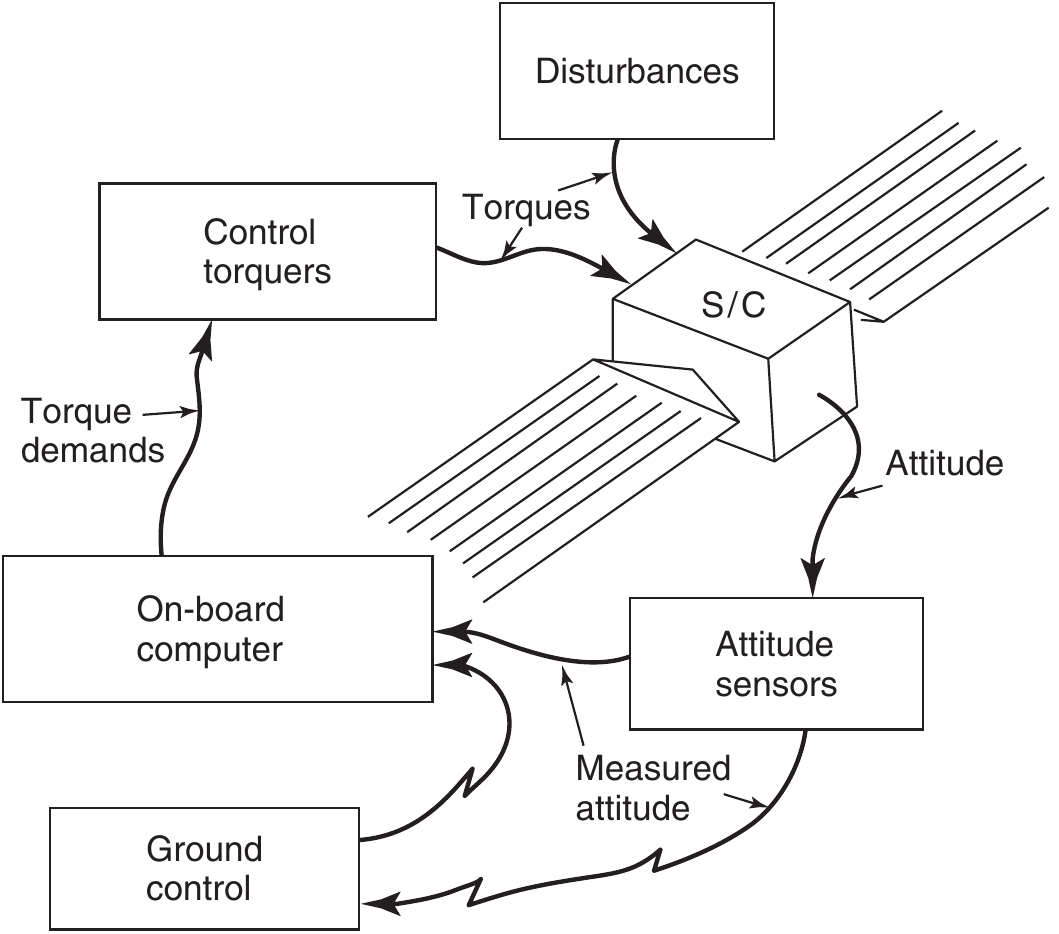
\includegraphics[width = 0.6\textwidth]{ACSblockdiag.png}
	\caption{Block diagram representing the ADCS \cite{SSE}.}
	\label{fig:acsblockdiag}
\end{figure}
\clearpage
\section{Experimental methods to assert pointing requirements}
In this section, the experimental procedure used to test the precision of the photometric methods is described. 

\subsection{Experimental setup}\label{sect:diffsetup}
The goal of the experimental design was to produce two spots of light on the CCD plane simulating stars. This is to analyze the stability with respect to small fluctuations in the pixel position of the light centroid. 

The setup is seen in figures \ref{fig:diffsetup} and \ref{fig:diffsetup2}. It comprises the detector in question, a tip-tilt mirror, and a light source that generates the two spots. The two spots are generated using a cardboard box with one open end. Inside the box a compact fluorescent lightbulb (CFL) was mounted and connected to the main relay. There were several options for different light bulbs, and this particular type of bulb was chosen to mimic the original experimental setup used in the characterization procedure. The open end of the cardboard box is covered in a thick piece of aluminum foil, in which two appropriate holes are poked with a needle. This created two light sources imaged at the detector. The tip-tilt mirror allows for adjustment of the position of the spots on the CCD. 

\subsection{Experimental procedure and data analysis}
Initially, an acquisition of several hours  was initiated (500 images of 40 second exposure time, with an idle time of 60 seconds between each acquisition). At first the mirror was not adjusted. Very small fluctuations are observed. These may be due to thermal fluctuations in the tip-tilt screws, or vibrations in the floor from people walking in the adjacent hallway. The centroid movement on the CCD is on the sub-pixel level. This sub-pixel movement emulates the movement of stars imaged on the detector, as the satellite pointing is never completely stable. 

\subsubsection{Data analysis}
After having acquired the data set, in each image, we should first apply necessary corrections to the image. These are subtraction of the bias frame, and application of a flat-field and hot pixel correction. The latter two are important such that we do not mistake positional flux variations for those stemming from flat field errors that are correctable. We should also know the readout noise levels in the detector, which is important when accounting for the noise budget. This is outlined in the next section. After correcting the image, we then apply aperture photometry to both spots, enabling us to estimate the flux in ADU for each aperture, after subtraction of the background found by using the corresponding annulus. The differential flux is then given as
\begin{equation}
	\Delta\bm F_i = \frac{\bm F_{i, 1}}{\bm F_{i, 2}}
\end{equation}
where $\bm F_{i, 1}$ is the flux in the $i$'th image, in the first aperture, and so on, estimated using aperture photometry as specified in \ref{sect:apphotmeth}. An overview of the movement of the centroid in both the $x$- and $y$- positions as a function of time is needed, as well as the differential flux as a function of time. These three data series may be plotted side by side, as is seen in \ref{fig:fluxposvtimecorr_atikcam}. 

\begin{figure}[h!]
	\centering
	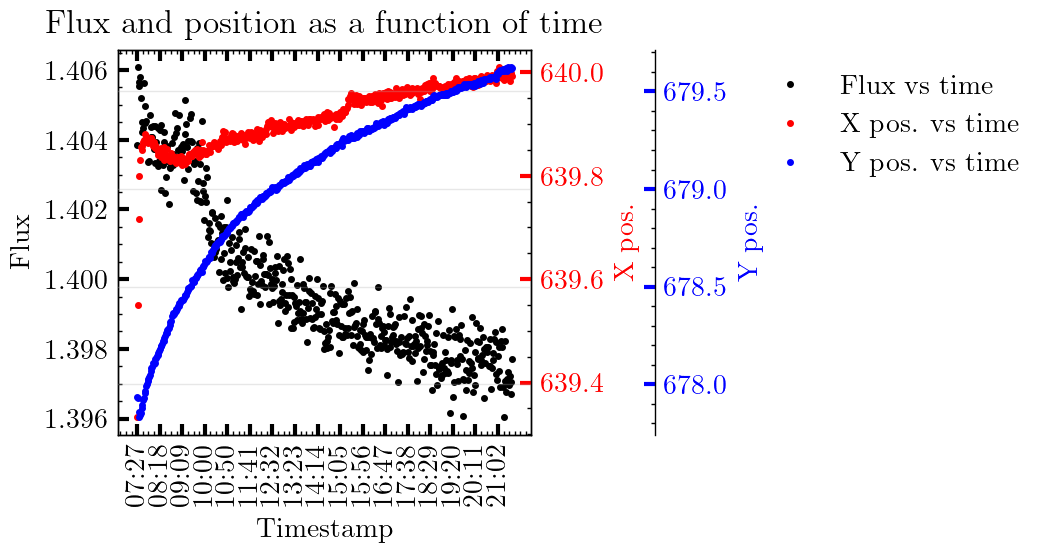
\includegraphics[width = 0.99\textwidth]{fluxposvtimecorr_atikcam_1.png}
	\caption{A plot showing the differential flux measured as a function of time (with black), the x- (with red), and y- (with blue) positions of the found centroid of the light, in pixel numbers.}
	\label{fig:fluxposvtimecorr_atikcam}
\end{figure}

\pagebreak
\begin{figure}[hbt!]
	\centering
	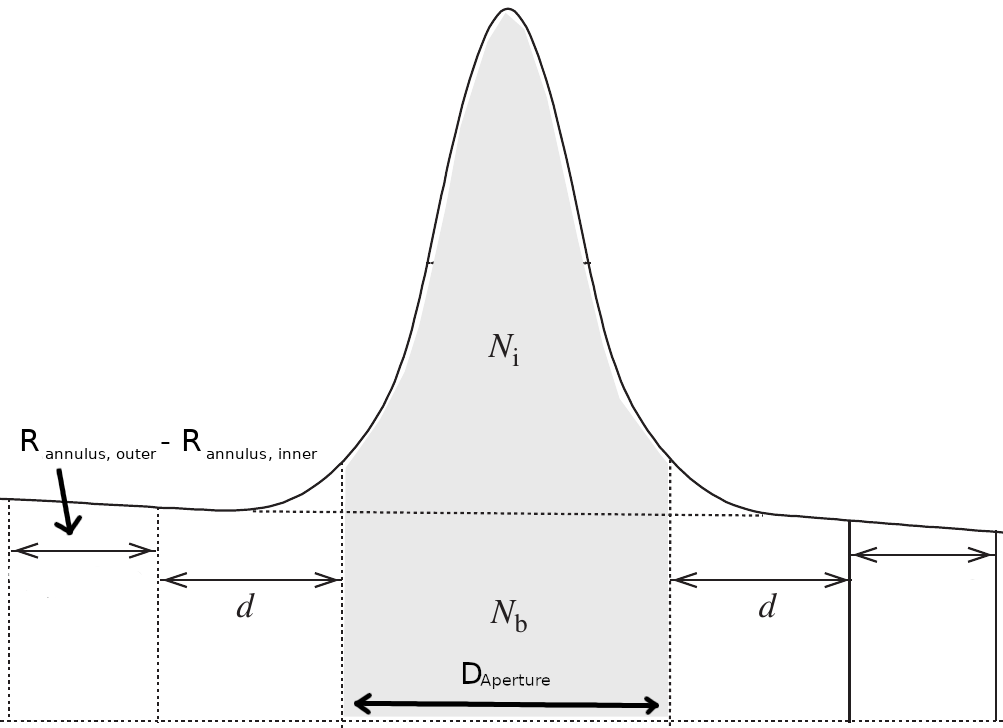
\includegraphics[width	=0.99\textwidth]{shotnoisebackground.png}
	\caption{A depiction of the situation analyzed in section \ref{sect:shotnoise_missionreq}, where a signal peak is situated on top of an arbitrary background. This is a modified figure from \cite{noisefigbookdetector}. The situation in question is the crosssection of the aperture, in which a light spot is a distribution of counts around some centroid. Naturally in the image, the distribution is two-dimensional (but otherwise assumed to be symmetric). The distribution follows counting statistics. Within the region of interest, denoted by a width $D_\text{aperture}$, which is the diameter of the chosen aperture, $N_i$ is a quantity denoting the counts of interest. This is the true signal from the light spot. $N_b$ denotes the counts in the background. At some distance $d$ the annulus is defined by an inner and outer radius, respectively $R_\text{annulus, inner}$ and $R_\text{annulus, outer}$. The annulus is used to approximate the background counts in the region of interest, $N_b$.}
	\label{fig:shotnoisebackground}
\end{figure}
\pagebreak
\section{Accounting for noise budgets}\label{sect:shotnoise_missionreq}

We should take great care and ensure that the noise levels observed in the differential flux, are accounted for by the photonic- and readout noise. Otherwise, we cannot be sure if the flux changes we observe are due to movements and not noise.

In section \ref{sect:photonicnoise}, photonic noise was described. In this section, we shall study the contribution of photonic noise, to the differential flux, as we move spots on the CCD. We use aperture photometry to estimate background noise, and single out the signal due to the incoming flux of light from a light source. An expression for the total photonic noise contribution to the differential flux will now be derived. 

Consider first figure \ref{fig:shotnoisebackground}. A signal peak is located on top of a background. This situation is the cross-section of the case on the CCD. The two spots are smeared out. We can think of the intensity in the spots as a two-dimensional distribution (gaussian in the ideal case), resting on top of a distribution of noise. $D_\text{aperture}$ is the diameter of the aperture, while the radii $R_\text{annulus, inner}$ and $R_\text{annulus, inner}$ define the annulus. The quantities $A_\text{aperture}$ and $A_\text{annulus}$ are the areas of the aperture and annulus respectively. The former area constitutes the region of interest, and the signal of interest, in counts of photons (ADU or generated electrons), is denoted in this case by $N_i$ is defined by this area. The latter area, $A_\text{annulus}$ is used as a local approximation to the noise level inside the aperture and is situated at a distance $d$ from the aperture. All of this is consistent with the top-down view of the analogous situation in figure 
\ref{fig:aperture}, and these quantities may be generalized to the two-dimensional case at hand. 

If we define a quantity $N_t$ as the total number of counts inside the region of interest, and $N_\text{annulus}$ to be the counts in the annulus used to define $N_b$ then clearly
\begin{equation}
	N_i = N_t - N_b = N_t - N_\text{annulus}\frac{A_\text{aperture}}{A_\text{annulus}}
\end{equation}
by use of error propagation we can obtain the error in the measurement of $N_i$ as $\sigma_i / N_i$ (as photonic noise is poissonian), where
\begin{equation}
	\sigma_i = \sqrt{\sigma_t^2 + \sigma_\text{annulus}^2\left(\frac{A_\text{aperture}}{A_\text{annulus}}\right)^2}
\end{equation}
Here $\sigma_t = \sqrt{N_t}$ and $\sigma_\text{annulus} = \sqrt{N_\text{annulus}}$ due to poisson statistics. Substituting these, and the definition of $N_t$ we get
\begin{equation}
	\sigma_i = \sqrt{N_i + N_\text{annulus}\left( \frac{A_\text{aperture}}{A_\text{annulus}}\right) + N_\text{annulus}\left( \frac{A_\text{aperture}}{A_\text{annulus}}\right)^2}
\end{equation}
We should take into account the total readout noise in one aperture and annulus $\sigma_\text{$i$, RON}$, by including $\sigma_\text{RON, pixel}$, electrons introduced per pixel during read out of the image. This can be done analogously such that
\begin{align}
	\sigma_\text{$i$, total}^2 = \sigma_i^2 &+ \sigma_\text{$i$, RON}^2 \\\nonumber= N_i &+ N_\text{annulus}\left( \frac{A_\text{aperture}}{A_\text{annulus}}\right)\left(1+ \frac{A_\text{aperture}}{A_\text{annulus}}\right) \\ &+ A_\text{aperture}\sigma^2_\text{RON, pixel} + A_\text{annulus}\sigma^2_\text{RON}\left(\frac{A_\text{aperture}}{A_\text{annulus}}\right)^2\nonumber
	\\ = N_i &+ N_\text{annulus}\left( \frac{A_\text{aperture}}{A_\text{annulus}}\right)\left(1+ \frac{A_\text{aperture}}{A_\text{annulus}}\right) + A_\text{aperture}\sigma^2_\text{RON, pixel}\left(1+ \frac{A_\text{aperture}}{A_\text{annulus}}\right)\nonumber
\end{align}
Where the second to last term is the readout noise in the aperture, and the last term is the contribution from readout noise in the annuli when subtracting the background. The total noise contribution in an aperture, taking into account the background by using the annuli, is then given by $\sigma_{i, \text{total}}/N_i$. The noise in both apertures will contribute to the noise levels in the differential flux, so we must compute 
\begin{equation}
	\sigma_\text{diff. flux} = \textbf{Noise level in differential flux} = \sqrt{\left(\frac{\sigma_{1,\text{total}}}{N_1}\right)^2 + \left(\frac{\sigma_{2,\text{total}}}{N_2}\right)^2}
\end{equation}
Thus we may calculate the noise level in an image, and doing this for the entire differential flux time series we may find a mean value.

We may then compare this value to the standard deviation of the differential flux data series, after having transformed any linear trends away. This can be done in the following way
\begin{equation}\label{eq:datatransform}
	\Delta \bm F'_i = \Delta \bm F_i - \frac{\Delta \bm F_{i-1} + \Delta \bm F_{i+1}}{2}
\end{equation}
Where $\Delta \bm F'_i$ is the transformed datapoint of the differential flux, and $\Delta \bm F_i$ is the $i$'th datapoint of the differential flux time series. We may then compare the standard deviation of this data series to that of the photonic noise calculated, noting that the standard deviation of the transformed data series has increased by a factor of $\frac32$, which should be accounted for as well. The data in question may be seen, after cutting a few data points in the beginning to avoid wild jumps, and after the transformation in eq. (\ref{eq:datatransform}), in figure \ref{fig:fluxposvtimecorr_atikcam_transform}. The jumps are probably caused by disturbances caused by being in the room, walking around, or sitting at the desk. The configuration with the tip-tilt mirror, seems to be very sensitive.

For the Atik 414EX detector, the relative photonic noise is computed to be $ \sigma_\text{diff. flux} = 0.00040 $ and the standard deviation of the transformed differential flux, seen in figure \ref{fig:fluxposvtimecorr_atikcam_transform}, is $\sigma_\text{trans. flux} = 0.00041  $. We have thus completely accounted for the noise levels, and the resulting change in flux as a function of the movement, as observed in the flux curve of figure \ref{fig:fluxposvtimecorr_atikcam}, is truly due to the movement of the light centroid on the chip. 

\begin{figure}[h!]
	\centering
	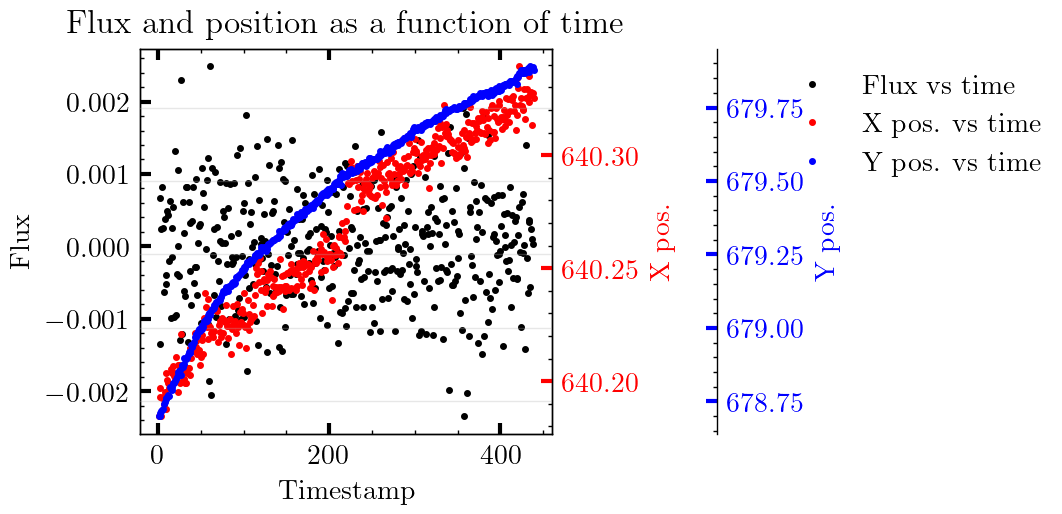
\includegraphics[width = 0.99\textwidth]{fluxposvtimecorr_atikcam.png}
	\caption{The same as in figure \ref{fig:fluxposvtimecorr_atikcam}, but after the data for the differential flux has been transformed to leave only noise. The data series has been cut in the beginning to avoid the wild fluctuations in the x-position. These jumps seem to be due to the system having to settle initially. This may be due to disturbances caused by sitting at the desk or likewise. The system seems to be very sensitive to disturbances. Now the flux is entirely noise, which we may compare with the photonic and readout noise levels to ensure that we can account for the entirety of the noise. }
	\label{fig:fluxposvtimecorr_atikcam_transform}
\end{figure}


\newpage
\begin{figure}[h!]
	\centering
	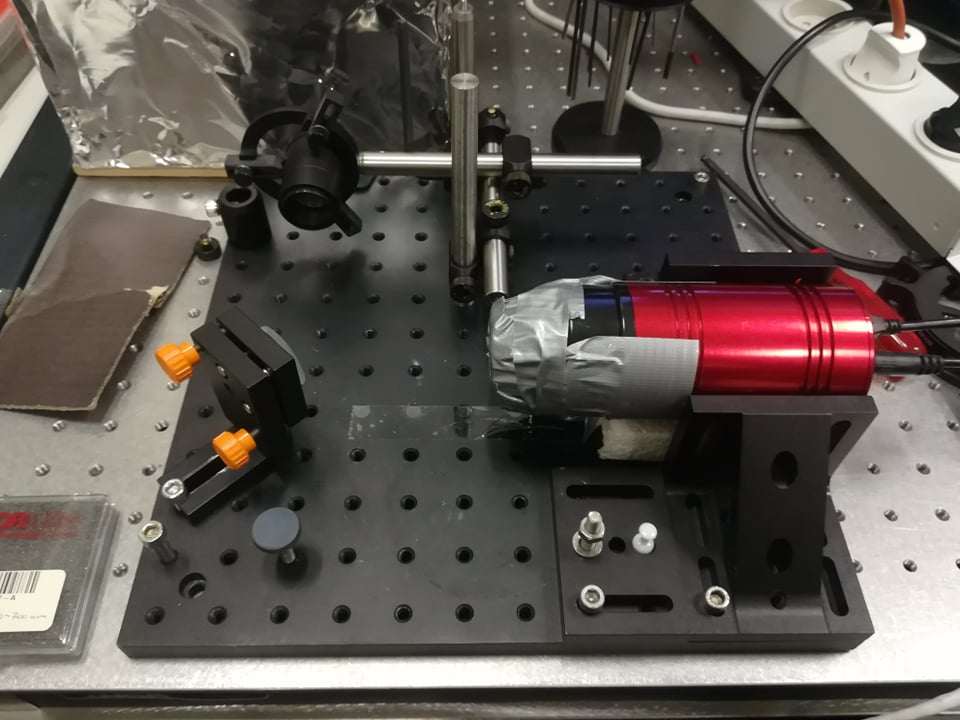
\includegraphics[width = 0.99\textwidth]{diffsetup3.jpg}
	\caption{An overview of the experimental setup used to perform the pointing stability test. The Atik 414EX detector is seen on the right side of the image, pointed at a tip-tilt mirror. In the back (upper left corner) the light source can be seen. In between the tip-tilt mirror and the tin foil, a mount for a lens is seen, but this was not used as it proved to be unnecessary.}
	\label{fig:diffsetup}
\end{figure}
\newpage
\begin{figure}[h!]
	\centering
	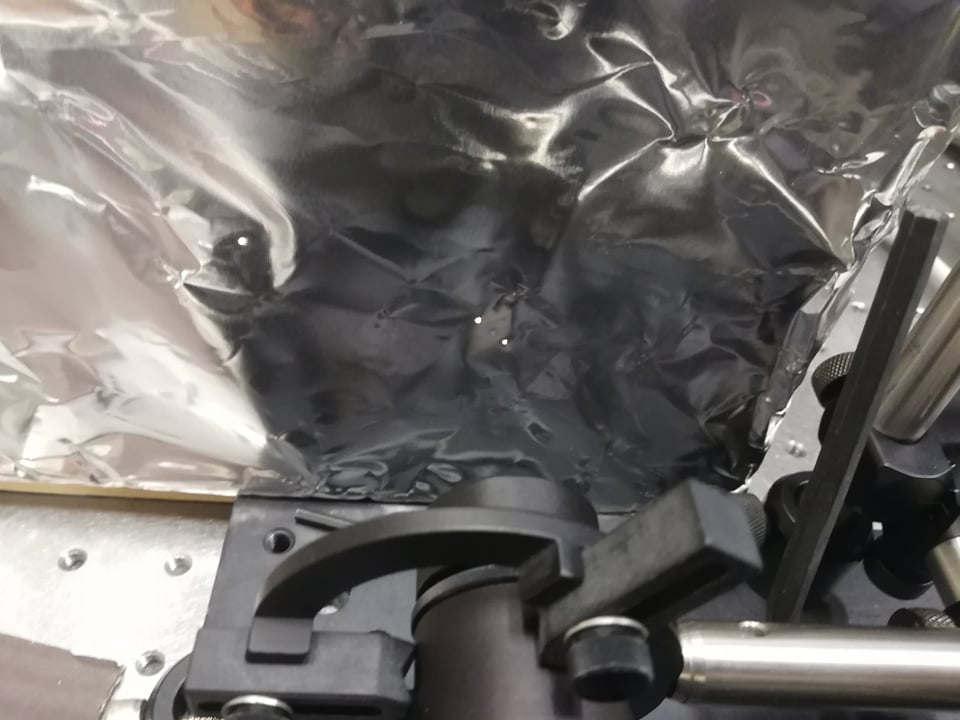
\includegraphics[width = 0.99\textwidth]{diffsetup4.jpg}
	\caption{A close up of the light source in the setup (see figure \ref{fig:diffsetup}), where the two spots may be clearly seen in the tin foil.}
	\label{fig:diffsetup2}
\end{figure}
\newpage

%\begin{figure}[h!]
%	\centering
%	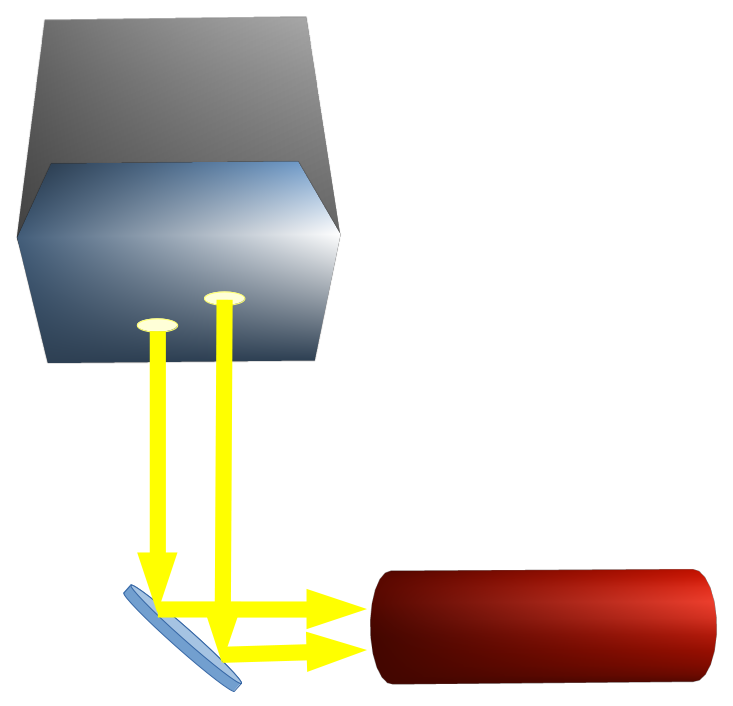
\includegraphics[width = 0.4\textwidth]{diffsetup_3d_illustration.png}
%	\caption{}
%	\label{fig:diffsetupIll}
%\end{figure}


\section{Results and technical specifications from scientific requirements}\label{sec:secondreq}
\begin{figure}[h!]
	\centering
	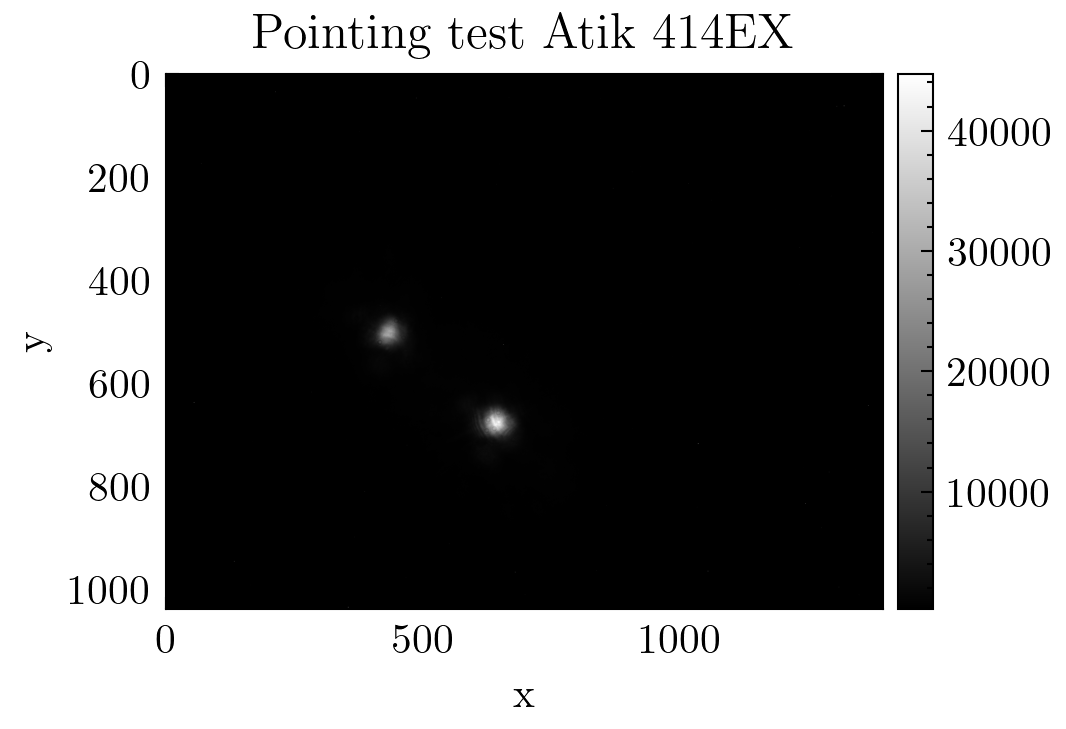
\includegraphics[width = 0.8\textwidth]{pointingtest_atik.png}
	\caption{A plot of the two light spots generated by the setup, imaged onto the CCD plane.}
	\label{fig:atikspots}
\end{figure}
In the preceding section, it was concluded that the trend observed in the flux curve of figure \ref{fig:fluxposvtimecorr_atikcam} is truly due to the movement of the light centroid on the chip, as we could account for the small variations in the curve by noise computations. That means we can plot the differential flux on the chip as a function of position and observe a functional trend. The variation of the flux, as a function of position, may be seen, plotted as a deviation from the initial data point, in figure \ref{fig:fluxvsPosatik}. A clear linear trend is observed, and a linear function $\bm F(x) = ax + b$ is fitted, where $\bm F$ is the flux. For the Atik 414EX detector, as depicted in the figure, the coefficients are computed to be $a_x = -2.238,\;b_x =  1431.839,\;a_y = -0.356,\;b_y =  241.295$. We may use this to establish a technical requirement from the mission requirement that the flux change is to be constrained to $\Delta F_\text{diff.} = 0.1 \%$ (as for the Kepler mission), by using that 
\begin{equation}
	\Delta x = \frac{\Delta F_\text{diff.}}{a_x}
\end{equation}
and likewise for the movement in the y position. For the the Atik 414EX detector, the conclusion is that we may at most move 
\begin{equation}
	\Delta x =  0.045 \;\text{pixels}, \quad
	\Delta y =  0.281 \;\text{pixels}
\end{equation}
which is a direct input to the technical requirements posed on the satellite ADCS system. The sensitivity to movements is significantly lower in the $y-$direction. This may be due to the construction of the CCD. If the $y-$direction is the readout direction, then movements along this direction will be along a photosensitive region (the buried columns/channels of photoactive silicon). Movements in the transverse direction will move the spot further into the non-sensitive region between the columns (see figure \ref{fig:ccdreadreg}).

We wish to interpret this result in terms of a general movement, instead of one that depends on the direction. The squared mean is computed as a measure of the allowable movement
\begin{equation}
	\text{Squared mean} =  \overline{\Delta r} = \sqrt{\frac{\Delta x^2 + \Delta y^2 }{2}} = 0.20126\; \text{pixels}
\end{equation}
Depending on the telescope that will be flown with the detector, movements (in pixels) on the chip, can be related to angular pointing requirements. 
\begin{figure}[h!]
	\centering
	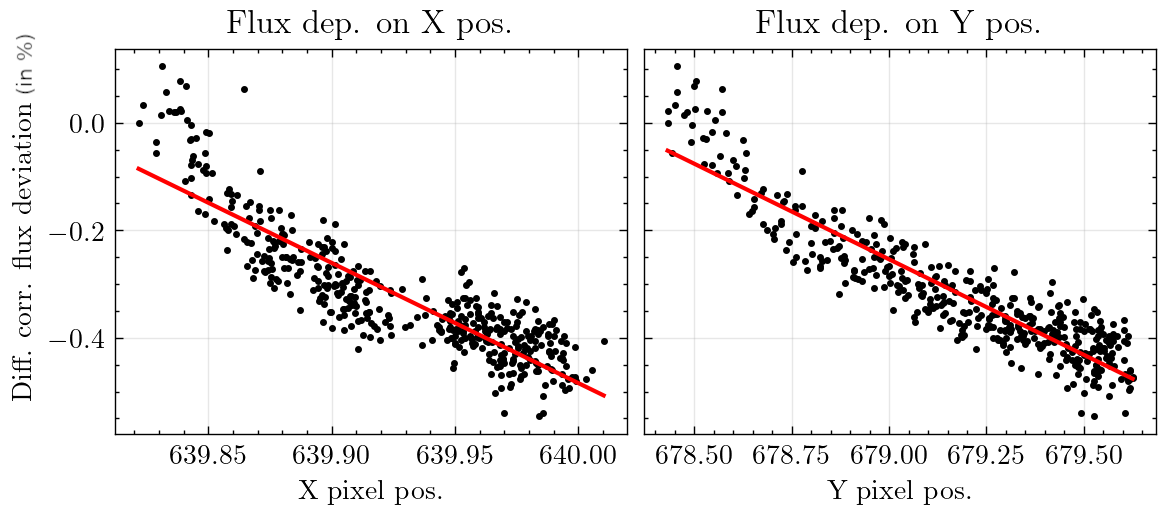
\includegraphics[width = 0.99\textwidth]{fluxvsposatik.png}
	\caption{The deviation (from the flux in the first datapoint) in the differential flux (in percentage) as a function of pixel positions in the X and Y directions on the CCD. Initially the datapoints are further from the line, likely due to the systems sensitivity to external disturbances, as those discussed in the text of figure \ref{fig:fluxposvtimecorr_atikcam_transform}. A linear function, $f(x) = ax + b$, of the movement has been fitted to the flux. Found coefficients are $a_x = -2.238,\;b_x =  1431.839,\;a_y = -0.356,\;b_y =  241.295$. This linear function is what yield technical specifications from the input scientific requirements.}
	\label{fig:fluxvsPosatik}
\end{figure}
\clearpage
\section{Measurement plan}\label{sec:attmeasplan}
In this section, a measurement plan will be provided, such that the test procedure to determine the pointing requirements, may be exactly reproducible. This measurement plan relies on the completion of the characterization procedure using the measurement plan of the last chapter. This is crucial as knowledge of the readout noise level, as well as the construction of both the flat field and bias frames as well as the hot pixel mask, are important for the data analysis.

\begin{enumerate}
	\item \textbf{Preparation:} 
	\begin{itemize}
		\item Perform the characterization procedure of the detector as described in section \ref{sec:charmeasplan}. In particular, the steps relating to the noise levels, frame and mask corrections are important prerequisites
	\end{itemize}
	\item \textbf{The experimental setup:} 
	\begin{itemize}
		\item The setup should consist of a modality that results in very small fluctuations of the light centroid on the detector. The light spots were defocused in the experiment described above, and no focusing lens was used. For the experiment described above a small tip-tilt mirror was used, and natural variations were observed as a result
		\item Two point sources of light may be constructed by using holes in tin foil in front of a light source.
	\end{itemize}
	\item \textbf{Data acquisition:}
	\begin{itemize}
		\item The exposure time used to acquire images should be chosen such that the mean ADU in an image falls in the linear range of the detector dynamic range. In this range the linearity is of the desired photometric precision should be as stated in the mission requirements.
		\begin{itemize}
			\item Considering, for the Atik 414EX detector, figure \ref{fig:linearitydim}, the $[1*10^4, 2*10^4]$ ADU range is well correlated and linear, to a precision of $10^{-4}$.
			\item For the Atik 414EX detector, an exposure time of $40$s in this light setting, falls in this ADU range, and this exposure time was chosen.
		\end{itemize}
		\item Acquire a series of images in a dark room of the two spots, in a period of a few hours. For the Atik 414EX detector, $N=500$ images were acquired, using a $40$s exposure time, and a $60$s idle time in between each image. This corresponds to a measurement series acquired over a timespan of $\sim 14$hrs, allowing the light spots enough time to move a significant distance on the detector face.
	\end{itemize}
	\item \textbf{Data analysis:}
	\begin{itemize}
		\item For each image acquired, perform a bias frame subtraction, then a flat field correction, and lastly a hot pixel correction
		\item Calculate the flux in each of the two spots using aperture photometry as described above in section \ref{sect:apphotmeth}. The differential flux is computed by focusing on one of the spots, calculating the relative flux as described in \ref{sec:diffphot}.
		\item Compute the positions of the centroids for each acquisition.
		\item The differential flux may then be plotted as a function of time, along with the positions of the centroid of the chosen spot, as a function of time.
		\item Before an estimate of the total noise contribution is calculated, transform the differential flux data set as described by equation (\ref{eq:datatransform}).
		\item Compute the total shot noise level in the data set using the method described in section \ref{sect:shotnoise_missionreq}. This value must be compared to the standard deviation of the transformed differential flux as a function of time that was constructed in the former step. If these two values are roughly equal we may account for the noise levels, and the changes in the differential flux, is attributed to movements of the centroid on the chip.
		\item Fit a linear function to the differential flux level deviations as a function of centroid position. Inputting the mission requirement as a maximum allowable flux change yields the technical requirement on the allowable movement of the centroid of the chip as an output. 
	\end{itemize}
\end{enumerate}

\clearpage
\section{Proof of concept: Testing the Prosilica GC660M camera}

For proof of concept, the AVT Prosilica GC660M camera will be taken through the test procedure above, ensuring that we reproduce sensible results. 

\begin{figure}[h!]
	\centering
	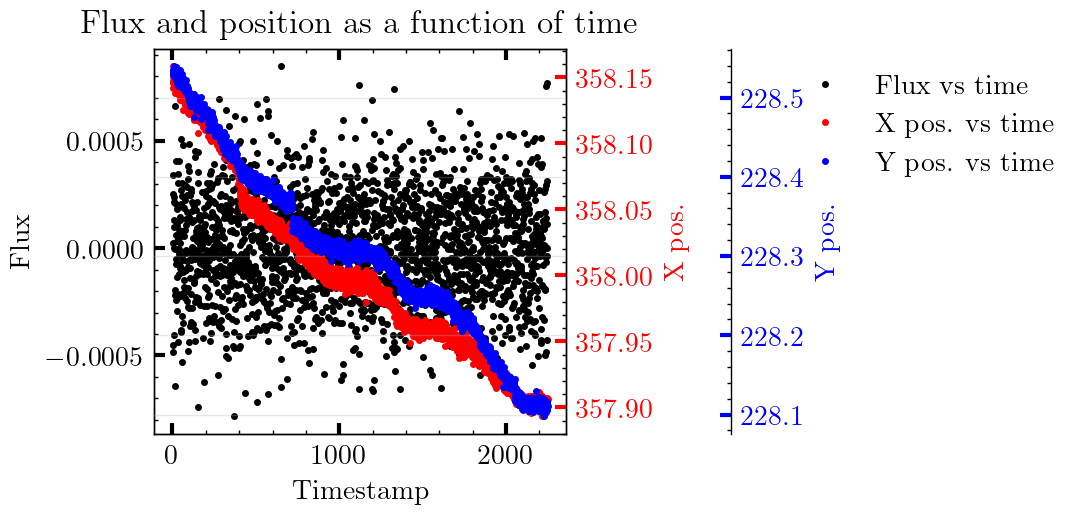
\includegraphics[width = 0.99\textwidth]{fluxposvtimecorr_AVT.png}
	\caption{The same as in figure \ref{fig:fluxposvtimecorr_atikcam_transform}, but for the AVT Prosilica GC660M camera. }
	\label{fig:fluxposvtimecorr_AVT_transform}
\end{figure}

\subsection{Preparations and experimental setup}
The setup used is the same as that for the Atik 414EX detector, and the characterization procedure was performed above and described in section \ref{sec:avtchar}. 

\subsection{Data acquisition}
The chosen exposure time was $5$ seconds, ensuring a mean ADU value in each spot of $\sim 1500$ ADU, which is in the middle of the linear range, as can be seen in figure \ref{fig:avtlinearity}. A series of images, $N=4000$ were acquired, and the last $2250$ frames were used to conduct the analysis. The series was cut short as there was a large jump in both the $x$ and $y$ positions in the first third of the dataset that there is no satisfactory explanation for. An idle time of $60$s was chosen, just as for the Atik 414EX detector.

\begin{figure}
	\centering
	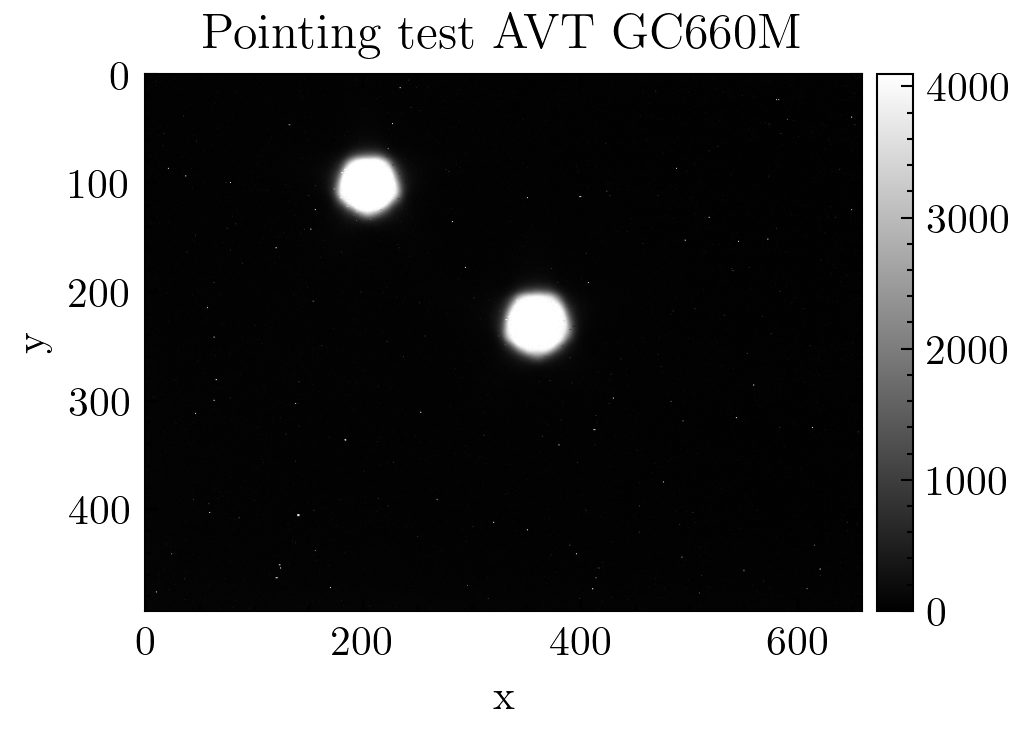
\includegraphics[width	=0.8\textwidth]{pointingtest.png}
	\caption{The two light spots, as imaged by the AVT Prosilica GC660M camera. Cf. figure \ref{fig:atikspots}, it is seen that the spots are significantly more defocused on the AVT Prosilica GC660M detector plane.}
	\label{fig:apertureAVT}
\end{figure}

\begin{figure}
	\centering
	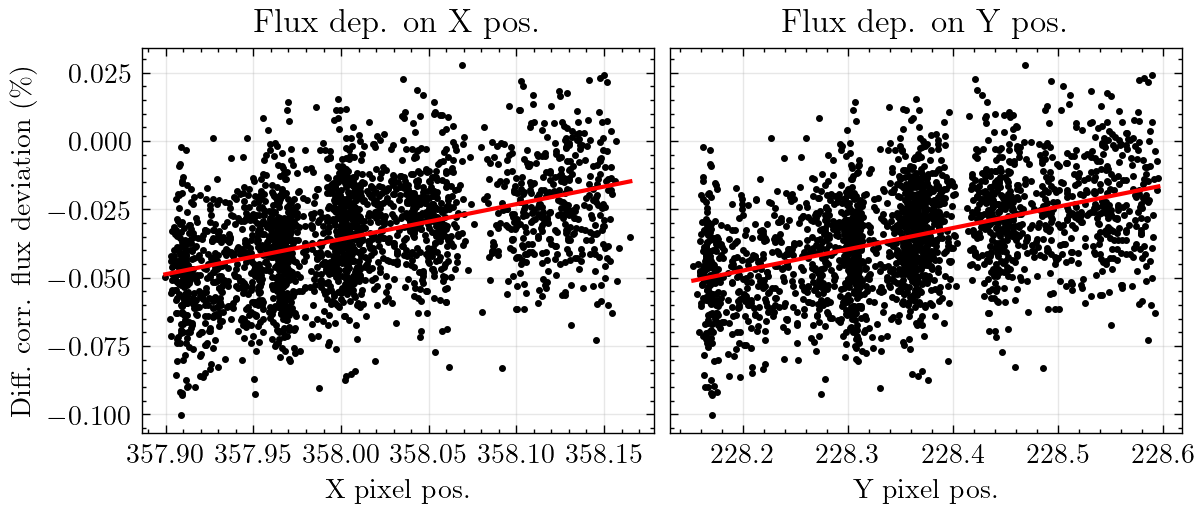
\includegraphics[width = 0.99\textwidth]{fluxvsposAVT.png}
	\caption{The same as in figure \ref{fig:fluxvsPosatik}, but for the AVT Prosilica GC660M camera. Found coefficients are $a_x = 0.128,\;b_x =  -45.883,\;a_y = 0.077,\;b_y = -17.813$.}
	\label{fig:fluxvsPosAVT}
\end{figure}

\subsection{Data analysis}
Figures \ref{fig:fluxposvtimecorr_AVT_transform} and \ref{fig:fluxvsPosAVT} show the result of the data analysis applied to the AVT camera. The total noise, following section \ref{sect:shotnoise_missionreq} was computed to be $0.000184$, and the standard deviation of the transformed differential flux data series (plotted in figure \ref{fig:fluxposvtimecorr_AVT_transform}) was computed to be $0.000173$, and we may hence account for the noise. A linear fit to the flux as a function of movement, seen in figure \ref{fig:fluxvsPosAVT} yields the coefficients $a_x = 0.128,\;b_x =  -45.883,\;a_y = 0.077,\;b_y = -17.813$, and consequently we find that the allowable movement is

\begin{equation}
	\Delta x =  0.781 \;\text{pixels}, \quad
	\Delta y =  1.285 \;\text{pixels}
\end{equation}
with allowable squared mean displacement
\begin{equation}
	\overline{\Delta r} = 1.00754 \;\text{pixels}
\end{equation}

which is a slightly looser criterion than that of the Atik 414EX detector. This may in part be explained by the spots being significantly more defocused on the image from the validation camera, seen in figure \ref{fig:apertureAVT} than they were on the image from the test procedure detector (as seen in figure \ref{fig:aperture}).

\clearpage
\section{Summary of results}\label{sec:attresults}
In this section, a brief summary of the results obtained in this chapter, will be presented in table \ref{table:pointingresults}.
% Please add the following required packages to your document preamble:
% \usepackage[table,xcdraw]{xcolor}
% If you use beamer only pass "xcolor=table" option, i.e. \documentclass[xcolor=table]{beamer}
\begin{table}[ht!]
	\centering
	\begin{tabular}{|
			>{\columncolor[HTML]{C0C0C0}}l ll|}
		\hline
		\multicolumn{3}{|c|}{\cellcolor[HTML]{C0C0C0}{\color[HTML]{000000} \textbf{Summary of Results}}}                                                                                                                                                                              \\ \hline
		{\color[HTML]{000000} \textbf{}}                                                                                     & \cellcolor[HTML]{C0C0C0}{\color[HTML]{000000} \textbf{Atik 414EX Mono}} & \cellcolor[HTML]{C0C0C0}{\color[HTML]{000000} \textbf{AVT Prosilica GC660M}} \\ \hline
		\multicolumn{3}{|c|}{\cellcolor[HTML]{C0C0C0}{\color[HTML]{000000} \textbf{Noise}}}                                                                                                                                                                                           \\ \hline
		\multicolumn{1}{|l|}{\cellcolor[HTML]{C0C0C0}{\color[HTML]{000000} \textbf{Total noise $\sigma_\text{diff. flux}$}}} & $0.00040$                                                               & $0.00018$                                                                    \\
		\multicolumn{1}{|l|}{\cellcolor[HTML]{C0C0C0}{\color[HTML]{000000} \textbf{Std. dev. $\sigma_\text{trans. flux}$}}}   & $0.00041$                                                               & $0.00017$                                                                    \\ \hline
		\multicolumn{3}{|c|}{\cellcolor[HTML]{C0C0C0}{\color[HTML]{000000} \textbf{Pointing req.}}}                                                                                                                                                                                   \\ \hline
		\multicolumn{1}{|l|}{\cellcolor[HTML]{C0C0C0}{\color[HTML]{000000} \textbf{$\Delta x$ {[}pixel(s){]}}}}              & $0.04468$                                                               & $0.74035$                                                                    \\
		\multicolumn{1}{|l|}{\cellcolor[HTML]{C0C0C0}{\color[HTML]{000000} \textbf{$\Delta y$ {[}pixel(s){]}}}}              & $0.28110$                                                               & $1.21745$                                                                    \\ 
		\multicolumn{1}{|l|}{\cellcolor[HTML]{C0C0C0}{\color[HTML]{000000} \textbf{$\overline{\Delta r}$ {[}pixel(s){]}}}}             
		& $0.20126$      
		& $1.00754$                                                                    \\ \hline
	\end{tabular}
	\caption{The results obtained in this chapter, tabulated.}
	\label{table:pointingresults}
	\end{table}

\end{document}